\chapter{Results of Experiments concerning \AspectOriented Modelling}
\label{chap:exp2_old_aspects_new_systems}
\label{chap:experimental_results}
\label{sec:optimisation_with_aspects_experimental_results}



The naive model of RPGLite and the \aspectoriented models of learning \&
confidence which are described in \cref{chap:experiment_setup} are designed to
answer the following research questions:

\begin{researchquestion}
  \begin{description}
\item[RQ2] \rqtwo{}
\item[RQ3] \rqthree{}
\item[RQ4] \rqfour{}
  \end{description}
\end{researchquestion}

% === Keeping this here for now --- think I might want to re-use it for talking
% === about the prior distribution model.
%To investigate these, the naive model of RPGLite play is augmented using the
%aspect-oriented models of learning outlined in
%\cref{sec:optimisation_with_aspects_aspectsdeveloped}. The datasets produced by
%executing both the unaltered naive model and the naive model with aspects
%applied are compared against the real-world dataset described in
%\cref{chap:rpglite}. Comparisons are made by quantifying the similarity of
%the character pair preferences found in each dataset as defined in
%\cref{measuring_charpair_similarity}. Whichever synthetic dataset is most
%similar to the empirically sourced one can be said to be the most realistic.
%This experiment has the null hypothesis that introducing aspects has no impact
%on model realism. If no change in model behaviour can be measured when learning
%models are applied, then it would be possible to \emph{represent} model changes
%as advice as demonstrated in
%\cref{sec:optimisation_with_aspects_aspectsdeveloped} but not possible to
%\emph{use} those changes in their aspect-oriented form.

To investigate each research question, relevant advice is woven into the naive
model, and datasets are generated of recorded simulated gameplay. To answer the
proposed research questions, these datasets are compared against the empirically
sourced datasets described in \cref{chap:rpglite}. Different experiments require
different comparisons and yield different contributions, but all make use of the
same foundations described in \cref{chap:experiment_setup}.

This chapter explores the results of the experiments which are enabled by the
previous chapter's foundations.
The first section describes how synthetic datasets are interpreted to yield
``optimal'' parameters when simulating a given player.
The second section explores an experiment answering the third research question,
concerning the use of advice to introduce new parameters and behaviours to a model.
The third section explores an experiment answering the fourth research question,
concerning the portability of advice as individual modules to new systems, or to
changed instances of the same system.
\inline{
  Add crefs to the sections mentioned here once they exist.
}


\section{Methodology concerning the Interpretation of Results}
\label{methodology_explained}

\subsection{K-Fold Validation}
\label{k_fold_validation_explanation}

RPGLite exhibits randomness, and its random nature affects the datasets
generated when running experiments; this may cause correlation to appear by
chance, biasing results. As discussed in
\cref{subsec:controlling_state_space_exploration}, efforts are made to mitigate
the impact of random play such as periodically refreshing the player pool and
ensuring many games are played. Efforts are also made when interpreting results
to control for the influence of random chance.

Simulations are run several times, and the datasets they generate are compared
against subsets of RPGLite player data to measure correlation, minimising the
impact of randomness when evaluating results. This is achieved using k-fold
validation, and ``Leave-One-Out Cross-Validation'' (LOOCV) in particular. In
k-fold validation, the dataset being compared against is divided into $k$
equally sized partitions (``folds''), which can be combined in different ways to
produce datasets for training an algorithm or finding optimal parameters for an
algorithm (``training~folds'') and corresponding datasets for testing the
results of each optimisation
(``testing~folds'')~\cite{k-fold-validation-definition}. LOOCV creates $k$ pairs
of training and testing folds, where testing folds are individual partitions,
and their corresponding training folds are the union of all other partitions.

All experiments in this chapter make use of LOOCV to minimise bias in results.
RPGLite player data is partitioned, and sets of training and testing folds are
produced from these partitions. Experiments generate multiple datasets,
comparing the results against different testing folds, and optimising model
parameters against different training folds where appropriate. In all
experiments \(k = 5\) to avoid small training \& testing folds and to measure
correlation many times, which helps to identify individual biased results.


\subsection{Identifying Model Parameters yielding Optimally Significant Results}
\label{identifying-significant-results-explanation}

\Cref{sec:rq2} and \cref{sec:rq3} describe experiments where parameters for the
model of learning are optimised. As this optimisation occurs across many folds,
it is possible that many parameters produce statistically significant datasets
when compared against a given player. These parameters may also vary between
folds, as comparison against different testing folds may show correlation with
different datasets. A technique to identify model parameters which produce
statistically significant results across many folds is therefore required.

Identifying optimal parameters requires searching across two dimensions of
statistical significance reported in experiment results: Kendall's \tau{}
correlation metric produces a statistic of correlation (which is also referred
to as \tau{} in the context of results) and a p-value describing the probability
that the correlation statistic would arise in the case that the null hypothesis
for a given experiment is true, as described in
\cref{measuring_charpair_similarity}. Statistically significant results must
demonstrate a sufficiently high correlation statistic and a sufficiently low
p-value; ``sufficiently'' high or low is defined below.

To identify parameters for a player which reliably produce statistically
significant results across folds, a threshold is set for both values of \tau{}
and their corresponding p-values. Parameters producing results which meet both
thresholds across $>50\%$ of folds are considered to be significant
parameters for simulating a player, as they are more likely than not to produce
datasets correlating to real-world play. If no such parameters exist,
thresholds are weakened, and the search repeats. Thresholds continue to be
weakened until doing so would indicate statistically insignificant results, such
as large p-value or a low \tau{} value. If no parameters exist which reliably
produce statistically significant results for a player, the player is not
accurately represented by the model.

\label{statistical_significance_thresholds_justified}
Correlation coefficient thresholds are selected at $0.5$, $0.4$, $0.3$, and
$0.2$. In behavioural science research, a correlation coefficient of $0.5$ is
considered strong in practice, $0.3$ of medium strength, and anything below
$0.2$ weak; these values are both suggested as
guidelines~\cite{significant_values_for_correlation_statistics} and found in the
distribution of published results in
metastudies~\cite{interpreting_correlation_coefficient_magnitude_psychology}. As
the model of learning used in these experiments predicts human behaviour,
typical bounds on high and low correlation from the behavioural science
community are adopted for these experiments, and a correlation coefficient below
$0.2$ is discarded in all cases as insignificant. P-value thresholds are $0.01$,
$0.02$, $0.035$, and $0.05$. A maximum value of $0.05$ is adopted by convention
in many research communities~\cite{borderline-significance-statistics-medicine};
other p-value thresholds are selected arbitrarily for incrementally more significant
results.

To determine which pairs are searched first, they are ordered by their Manhattan
distance from the most restrictive pair, $\tau{} > 0.5$ and $p < 0.01$. This is
calculated by summing the number of steps away from the most restrictive
threshold for each measurement: a threshold pair $\tau{} > 0.4$ and $p < 0.2$,
with a Manhattan distance of $1 + 1 = 2$, is considered stronger than a pair
$\tau{} > 0.5$ and $p < 0.05$, which has a Manhattan distance of $0 + 3 = 3$,
and therefore is used first when searching for significant results.

Experiments in \cref{sec:rq2} and \cref{sec:rq3} use this technique to find
``optimal'' parameters to model each player with statistical significance, if
such parameters exist for a player. The algorithm implementing this search is
given in \cref{search_for_correlation_coefficients} for reference.



\section{RQ2: Altering Model Behaviour using \AspectOrientation}
\label{sec:rq2}

\subsection{Experimental Design}

To demonstrate the viability of altering a model by using aspects to describe a
change in behaviour, the advice applying the already-known character pair
distribution to character pair selection is applied. This forms the first of
three experiments in this chapter, addressing the research question:

\begin{researchquestion}
\rqtwo{}
\end{researchquestion}

The research question yields a null hypothesis: \emph{models of systems cannot
be altered using advice to reflect their subjects more accurately}. If this were
the case, there would be no discernable difference between the real world data's
correlation against data from the naive model and data from a model with advice
woven. Simulated players in the naive model select character pairs randomly,
meaning that --- if patterns such as personal preference exist in the real-world
data, or the data is not randomly distributed --- we would not expect much
correlation between the two. If weaving advice produces datasets which do
correlate with the real-world data, then the advice would have affected the
model to more accurately reflect the player being simulated. We would therefore
discount the null hypothesis, and answer the research question affirmatively. If
no correlation could be produced as a result of weaving aspects, then the null
hypothesis would have been demonstrated instead, answering the research question
negatively.

\begin{figure}[h]
  \centering
  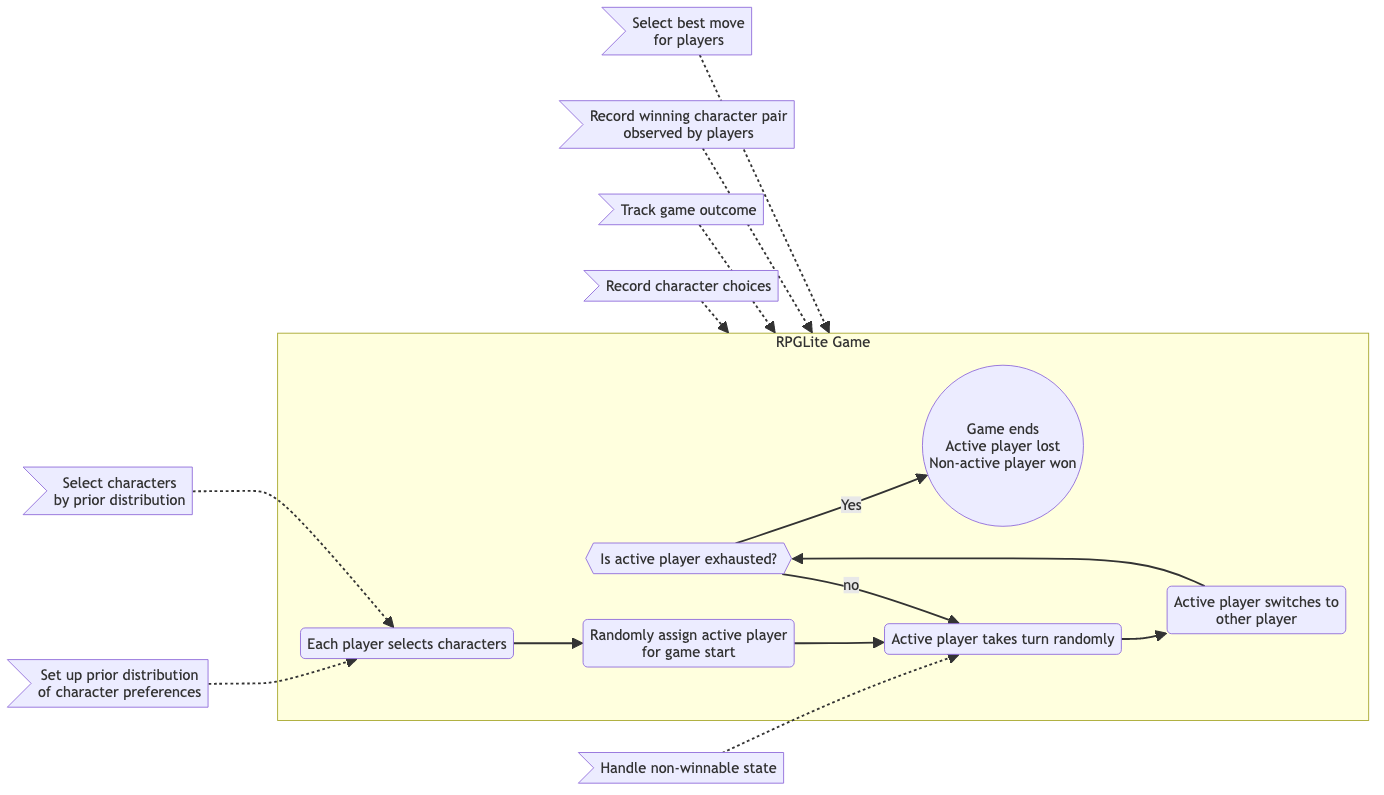
\includegraphics[width=\columnwidth]{70_generality_of_aspects/diagrams/exp2_prior_distribution_model.png}
  \caption{Advice woven into the naive model to adopt the distribution used to select character pairs from real-world data.}
  \label{fig:exp1_prior_distribution_model}
\end{figure}

\Cref{fig:exp1_prior_distribution_model} illustrates the advice woven into the
naive model to alter player behaviour to select character pairs with the same
distribution as the real-world data exhibits. As this advice causes simulated
players to select character pairs with the same distribution as real-world
players, the datasets generated using them ought to correlate strongly with the
real-world data: rather than being random, the distribution is expected to be
the same. This therefore tests our hypothesis that advice can be used to alter
model behaviour to be more accurate.
\footnote{
  Later experiments will investigate the addition of specific behaviours, rather
  than reproducing properties of an already-present dataset.
}


\subsection{Results}

Results are generated through k-fold validation as described in
\cref{k_fold_validation_explanation}. As no additional parameters are added to
the model, no searching for optimal parameters is required. A drawback of the
lack of searching for optimal parameters is that there is no convenient way to
summarise results across folds. However, results are \emph{consistent} across
folds; the result of the first fold is given in this section's result tables,
described below. Complete tables with data from all folds is given in
\cref{appendix-data-for-all-exp1-folds} in the interest of transparency. Results
are shown for players who completed at least $100$ games in season 1 of RPGLite,
and the experiment is conducted against season 1 gameplay data.

The results of the experiment are shown in
\cref{naive_model_results_table_comparison_to_real_world_datasets} for datasets
produced by the naive model, and
\cref{prior_distribution_results_table_comparison_to_real_world_datasets} for
datasets produced by applying advice to the naive model which alters the
distribution from which character pairs are selected. 

\begin{figure}[h]
  \centering
  
  \begin{minipage}{.45\textwidth}
    \centering
    \begin{tabular}{r|c|c}
      \emph{Username} & \emph{p-value} & \emph{\tau{} statistic} \\\hline\hline
    apropos0 & 0.930 & -0.013 \\
    basta & 0.182 & 0.205 \\
    creilly1 & 0.352 & 0.141 \\
    creilly2 & 0.764 & -0.046 \\
    cwallis & 0.042 & 0.309 \\
    Deanerbeck & 0.881 & -0.023 \\
    ECDr & 0.370 & 0.135 \\
    elennon & 0.683 & 0.062 \\
    Ellen & 0.417 & -0.120 \\
    Etess & 0.291 & 0.165 \\
    Fbomb & 0.169 & -0.220 \\
    Frp97 & 0.452 & 0.119 \\
    georgedo & 0.185 & 0.205 \\
    Jamie & 0.944 & -0.0106 \\
    kubajj & 0.704 & -0.058 \\
    l17r & 0.646 & -0.073 \\
    Nari & 0.330 & -0.152 \\
    Paddy & 0.294 & 0.166 \\
    sstein & 0.529 & 0.101 \\
    tanini & 0.213 & 0.185 \\
    timri & 0.160 & -0.220 \\
    \end{tabular}
    \caption{Correlation of real-world character pair selection and those generated by an unmodified naive model.}
    \label{naive_model_results_table_comparison_to_real_world_datasets}
  \end{minipage}\hfill
  \begin{minipage}{.45\textwidth}
    \centering
    \begin{tabular}{r|c|c}
      \emph{Username} & \emph{p-value} & \emph{\tau{} statistic} \\\hline\hline
      apropos0 & \scientific{6.070e-10} & 0.964 \\
      basta & \scientific{6.984e-09} & 0.975  \\
      creilly1 & \scientific{6.984e-10} & 0.961  \\
      creilly2 & \scientific{1.154e-08} & 0.984  \\
      cwallis & \scientific{2.514e-09} & 0.970  \\
      Deanerbeck & \scientific{4.742e-08} & 0.979  \\
      ECDr & \scientific{8.455e-10} & 0.959  \\
      elennon & \scientific{3.963e-09} & 0.973  \\
      Ellen & \scientific{2.538e-09} & 0.950  \\
      Etess & \scientific{1.113e-08} & 0.994  \\
      Fbomb & \scientific{3.117e-08} & 0.996  \\
      Frp97 & \scientific{2.440e-08} & 1  \\
      georgedo & \scientific{4.719e-08} & 0.970  \\
      Jamie & \scientific{5.760e-09} & 0.985  \\
      kubajj & \scientific{5.728e-09} & 0.966  \\
      l17r & \scientific{1.056e-07} & 0.994  \\
      Nari & \scientific{1.965e-08} & 0.985  \\
      Paddy & \scientific{1.171e-08} & 0.984  \\
      sstein & \scientific{5.017e-08} & 0.988  \\
      tanini & \scientific{1.539e-09} & 0.952  \\
      timri & \scientific{2.582e-08} & 0.990  \\
    \end{tabular}
    \caption{Correlation of real-world datasets of character pair selection and those generated by the naive model with advice woven to bias the characters chosen.}
    \label{prior_distribution_results_table_comparison_to_real_world_datasets}
  \end{minipage}

\end{figure}

Briefly summarised, the only player showing statistically significant results
from the data produced by the naive model is from \emph{cwallis}, from whom a
p-value of $0.042$ and a \tau{} correlation coefficient of $0.309$ is produced,
indicating medium-strength correlation with a low chance of being a coincidence.
As noted in \cref{identifying-significant-results-explanation}, a \tau{}
statistic above $0.2$ paired with a p-value below $0.05$ is the threshold set
for statistical significance.
With a 4.2\% chance of being coincidentally generated and 21 players simulated,
this outcome is not unexpected. Correlation results from \emph{cwallis}' other
folds show no significant correlation, as seen in the complete table presented
in \cref{appendix-data-for-all-exp1-folds}. The results of simulating all
players with advice woven show strong correlation and low p-values.


\subsection{Answering the Second Research Question}

The data shown in
\cref{naive_model_results_table_comparison_to_real_world_datasets} demonstrates
that --- without any advice woven into the model to alter its selection of
characters --- the naive model selects character pairs which do not correlate
with those found in real-world datasets at all. As the naive model acts randomly
with regards character pair selection, this aligns with expectations.

The data shown in
\cref{prior_distribution_results_table_comparison_to_real_world_datasets}
contains the correlation of real-world datasets for a player with the naive
model, with advice woven to select character pairs from the distribution found
in that player's empirical dataset. Every simulated player showed an
extremely strong correlation statistic and p-value for their simulated dataset's
correlation with their empirical equivalent. While this correlation is extreme,
it also matches expectations. Advice which selects character pairs using a known
distribution ought to result in that distribution being represented in
simulated games.

This demonstrates the hypothesised effect: player behaviour can be altered
though the weaving of aspects to produce a model which more closely matches
real-world observations in some manner. The research question can therefore be
answered affirmatively.

A curiosity of this experiment is that the altered behaviour is not a
cross-cutting concern as they are typically defined. Modularisation of these
parts of a program is \aop{}'s original use-case~\cite{kiczales1997aspect}, but
this experiment shows that the technique can be successfully used in other ways
(as suggested by \citet{gulyas1999use} and \citet{steimann06paradoxical}). The
success of advice as a mechanism to introduce change to a program, rather than
being used as a mechanism to refactor or more elegantly design it, suggests that
\aop{} could be well-suited to exaptation\footnote{\citet{exaptation_origin}
coined the term ``exaptation'' to refer to a trait of a species which evolved in
response to one need, but were later co-opted to satisfy another.} as a tool to
introduce new behaviours in a model.



\section{RQ3: Adding Model Behaviours \& Parameters using \AspectOrientation}
\label{sec:rq3}

\subsection{Experimental Design}

The behaviour added to the naive model in \cref{sec:rq2} impacts how accurately
the model reflects a player, but does not model new player \emph{behaviours}.
While this is sufficient to demonstrate that \aop{} can be successfully used to
improve a model, it does not answer the third research question:

\begin{researchquestion}
\rqthree{}
\end{researchquestion}

\revnote{
  I'm not satisfied with this motivation for this RQ and how it's isolated from
  the second RQ. Revisit this.
}

The experiment discussed in \cref{sec:rq2} changes the distribution used to
select characters, but does not parameterise its changes and adds no new
activity on the part of simulated players which would require a new parameter.
It therefore demonstrates that the software engineering technique can be applied
in the context of simulation \& modelling, but does not demonstrate that \aop
meets the needs of researchers who seek to apply advice which add or make changes to
the behaviours of actors in their simulations rather than tweaking existing
ones. As a result, answering this research question requires a further
experiment, which the \aspectoriented models of confidence and learning
introduced in \cref{chap:experiment_setup} yield.

\Aspectoriented{} models of confidence and learning are therefore woven into the naive model to
produce another in which players learn over time. A player's choice of
characters is not selected randomly from a distribution in this model, but
informed by their observations of wins and losses in previous games. The advice
used is that of the models of confidence and learning described in
\cref{chap:experiment_setup}. A diagram of the woven advice is given in
\cref{fig:learning_model_software_diagram}.

\begin{figure}[h]
  \centering
  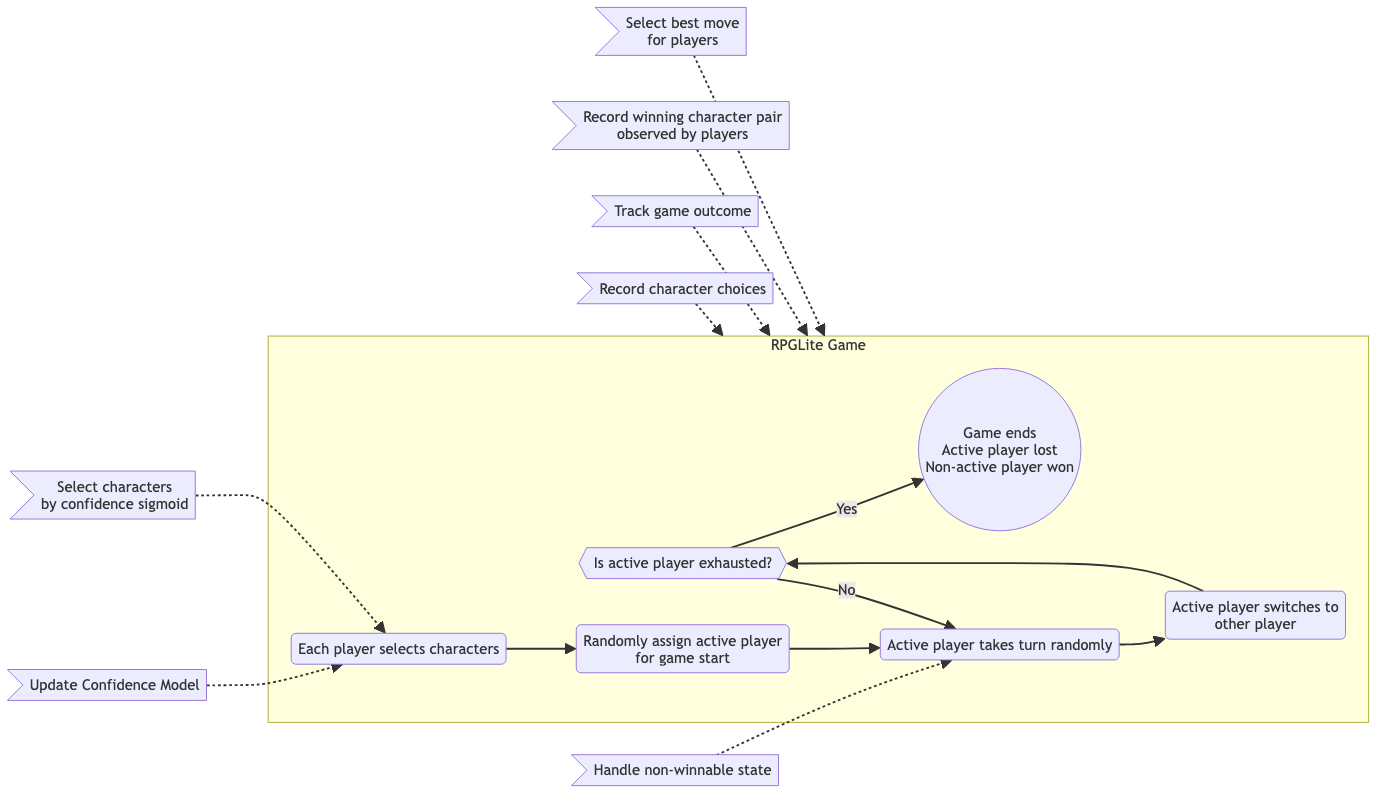
\includegraphics[width=\columnwidth]{70_generality_of_aspects/diagrams/exp3_learning_model.png}
  \caption{Advice woven into the naive model to amend simulated players' behaviour to include learning over time, and to track the relevant parameters for the related model of confidence.}
  \label{fig:learning_model_software_diagram}
\end{figure}

The null hypothesis associated with the research question this experiment
addresses is, \emph{advice cannot be used to accurately introduce behaviours or
parameters into a model in which they are not already present}. If this were
true, the datasets produced by the \aspectoriented model shown in
\cref{fig:earning_model_software_diagram} would exhibit no more correlation with
real-world data than the naive model does. If a learning behaviour can be
successfully introduced, some players' simulations would exhibit consistently
realistic behaviour which would correlate with their real-world data.

Unlike the experiment described in \cref{sec:rq2}, this experiment uses no
real-world data to inform the actions simulated players make. As a result, if
parameters can be found for a player which consistently generates datasets
correlating with their empirical dataset, the simulated player's behaviour must
have been successfully altered to learn in an accurate manner. This would
discount the null hypothesis; the research question could therefore be answered
affirmatively.




\subsection{Results}

Results were generated by running the naive model with advice woven which implements a
model of learning. Results were generated using k-fold validation and model
parameters searched for using the technique described in
\cref{identifying-significant-results-explanation}. The parameters modified when
running simulations were:

\begin{itemize}
  \item The confidence model's birch curve shape parameter, which could have any
  of the values $c \in \{\frac{1}{50}, \frac{1}{10},
    \frac{1}{5}, 1, 5, 10, 50\}$.
    \item The coefficient applied to scale the relative growth rate of the
    confidence model's birch curve, which could have any of the values $rgr
    ~ coeff. \in \{0.1, 0.3, 1, 3\}$
    \item The probability that a simulated player would become ``bored'' and
    replaced in the player pool for the simulation, as described in
    \cref{subsec:controlling_state_space_exploration}. The probability that a
    player would become bored could have any of the values $prob.~bored \in
    \{disabled, \frac{1}{64}, \frac{1}{16}, \frac{1}{4}, 1\}$
\end{itemize}

The results have been separated into two tables for
legibility: results for players for whom parameters could be found which produced statistically
significant correlation are shown in 
\cref{learning_model_results_table_comparison_to_real_world_datasets_correlating_players},
and results for players for whom no such parameters could be found are shown in
\cref{learning_model_results_table_comparison_to_real_world_datasets_players_without_correlation}.
For some players, many parameters could be found which produced correlating
data; in these cases,
\cref{learning_model_results_table_comparison_to_real_world_datasets_correlating_players}
contains all such parameters.Results
are shown for players who completed at least $100$ games in season 1 of RPGLite,
and the experiment is conducted against season 1 gameplay data.

\revnote{
  If there's time, consider making these results tables prettier, e.g. with the
  booktabs package as suggested in
  \href{https://tex.stackexchange.com/a/282930}{https://tex.stackexchange.com/a/282930}.
}

\begin{figure}[h]
  \centering
  
    \begin{tabular}{l|r|r|r|r|r|r}
      \emph{Username} & \emph{p-value <} & \emph{\tau{} >} &
\begin{tabular}{@{}c@{}}\emph{Confidence} \\ \emph{curve value}\end{tabular} &
\begin{tabular}{@{}c@{}}\emph{Confidence} \\ \emph{RGR modifier}\end{tabular}  &
\emph{Prob. bored} &
      \emph{\# folds}\\\hline\hline
apropos0 & 0.01 & 0.4 & 0.2 & 3 & 0.0625 & 3 \\
apropos0 & 0.01 & 0.4 & 10 & 0.1 & \emph{disabled} & 3 \\
cwallis & 0.01 & 0.4 & 0.02 & 0.1 & 0.25 & 4 \\
cwallis & 0.01 & 0.4 & 0.1 & 0.3 & 0.25 & 4 \\
cwallis & 0.01 & 0.4 & 1 & 0.1 & 0.25 & 4 \\
cwallis & 0.01 & 0.4 & 10 & 0.1 & 0.25 & 4 \\
elennon & 0.035 & 0.3 & 50 & 0.1 & 0.0625 & 3 \\
Ellen & 0.01 & 0.3 & 10 & 0.3 & 0.015625 & 3 \\
georgedo & 0.02 & 0.3 & 50 & 3 & 0.015625 & 3 \\
georgedo & 0.02 & 0.3 & 0.1 & 3 & 0.015625 & 3 \\
georgedo & 0.02 & 0.3 & 0.2 & 3 & 0.0625 & 3 \\
georgedo & 0.02 & 0.3 & 0.2 & 1 & 0.0625 & 3 \\
georgedo & 0.02 & 0.3 & 0.02 & 1 & 0.0625 & 3 \\
Jamie & 0.01 & 0.4 & 0.2 & 1 & 1 & 3 \\
Jamie & 0.01 & 0.4 & 1 & 3 & 0.25 & 3 \\
Jamie & 0.01 & 0.4 & 5 & 0.1 & 0.25 & 3 \\
Jamie & 0.01 & 0.4 & 0.02 & 1 & 0.015625 & 3 \\
    \end{tabular}
    \caption{Correlation of empirically sourced datasets and those generated by applying the \aspectoriented model of learning.}
    \label{learning_model_results_table_comparison_to_real_world_datasets_correlating_players}
  
\end{figure}

\begin{figure}[h]
  \centering
  
    \begin{tabular}{l|r|r|r|r|r|r}
      \emph{Username} & \emph{p-value <} & \emph{\tau{} >} &
\begin{tabular}{@{}c@{}}\emph{Confidence} \\ \emph{curve value}\end{tabular} &
\begin{tabular}{@{}c@{}}\emph{Confidence} \\ \emph{RGR modifier}\end{tabular}  &
\emph{Prob. bored} &
      \emph{\# folds}\\\hline\hline
basta & \emph{N/A} & \emph{N/A} & \emph{N/A} & \emph{N/A} & \emph{N/A} & \emph{N/A} \\
creilly1 & \emph{N/A} & \emph{N/A} & \emph{N/A} & \emph{N/A} & \emph{N/A} & \emph{N/A} \\
creilly2 & \emph{N/A} & \emph{N/A} & \emph{N/A} & \emph{N/A} & \emph{N/A} & \emph{N/A} \\
Deanerbeck & \emph{N/A} & \emph{N/A} & \emph{N/A} & \emph{N/A} & \emph{N/A} & \emph{N/A} \\
ECDr & \emph{N/A} & \emph{N/A} & \emph{N/A} & \emph{N/A} & \emph{N/A} & \emph{N/A} \\
Etess & \emph{N/A} & \emph{N/A} & \emph{N/A} & \emph{N/A} & \emph{N/A} & \emph{N/A} \\
Fbomb & \emph{N/A} & \emph{N/A} & \emph{N/A} & \emph{N/A} & \emph{N/A} & \emph{N/A} \\
Frp97 & \emph{N/A} & \emph{N/A} & \emph{N/A} & \emph{N/A} & \emph{N/A} & \emph{N/A} \\
l17r & \emph{N/A} & \emph{N/A} & \emph{N/A} & \emph{N/A} & \emph{N/A} & \emph{N/A} \\
kubajj & \emph{N/A} & \emph{N/A} & \emph{N/A} & \emph{N/A} & \emph{N/A} & \emph{N/A} \\
Nari & \emph{N/A} & \emph{N/A} & \emph{N/A} & \emph{N/A} & \emph{N/A} & \emph{N/A} \\
Paddy & \emph{N/A} & \emph{N/A} & \emph{N/A} & \emph{N/A} & \emph{N/A} & \emph{N/A} \\
sstein & \emph{N/A} & \emph{N/A} & \emph{N/A} & \emph{N/A} & \emph{N/A} & \emph{N/A} \\
tanini & \emph{N/A} & \emph{N/A} & \emph{N/A} & \emph{N/A} & \emph{N/A} & \emph{N/A} \\
timri & \emph{N/A} & \emph{N/A} & \emph{N/A} & \emph{N/A} & \emph{N/A} & \emph{N/A} \\
    \end{tabular}
    \caption{Correlation of empirically sourced datasets and those generated by applying the \aspectoriented model of learning for players who showed no correlation, separated for legibility.}
    \label{learning_model_results_table_comparison_to_real_world_datasets_players_without_correlation}
  
\end{figure}

Simulations of player \emph{cwallis} yielded 26 parameter combinations producing
statistically significant results, far more than any other player. For
legibility, only parameters which produced statistically significant correlation
in 4 folds are shown in
\cref{learning_model_results_table_comparison_to_real_world_datasets_correlating_players}.
A complete table with all results is provided in
\cref{appendix_complete_results_table_exp2}.


\subsection{Answering the Third Research Question}

\Cref{learning_model_results_table_comparison_to_real_world_datasets} shows that
six player are accurately modelled by the \aspectoriented model of learning
shown in \cref{fig:learning_model_software_diagram}. The answer to the research
question is therefore affirmative: advice can be used to accurately introduce
new behaviours and parameters to a model which were not previously present.

Not all players are accurately simulated using this model of learning. This
result is to be expected. One reason for this is that different players learn in
different ways; the model of learning developed in this thesis is not intended
to represent some universal model of learning (if such a model can exist) but to
represent some players' behaviours, thereby demonstrating that complex
behavioural models can be tractably modelled as advice. Another reason is that,
as these models draw from historically observed data, learning may be sensitive
to a player's personal biases: for example, they may not understand how to
usefully employ a certain character, skewing their observations of wins and
losses. Finally, real-world players may simply dislike certain characters for
superficial reasons, such as artwork or a lack of interest, which would skew
their distribution of character pair selections in a manner which the model of
learning would be unable to account for as written.

The accurate simulation of $\approx{}28.9\%$ of the sampled playerbase demonstrates two
successes of this experiment. First, the fact that model did not accurately
simulate \emph{all} players is a positive result: if it did, this would indicate
that the experiment was incorrectly conducted in some manner, as biases
unrelated to learning are to be expected in players' interactions with RPGLite,
making a 100\% success rate indicative of an error in the simulation. Second,
the research question is answered affirmatively: advice \emph{can} be employed
to represent new behaviours within -- and add new parameters to -- an existing model. 



\section{RQ4: Applying Aspects to New Models}
\label{sec:rq4}


\subsection{Experimental Design}

% The experiment in \cref{sec:rq2} is designed to demonstrate that tooling for
% \aspectorientation{} provided a \emph{viable} mechanism to alter a model; its
% successor in \cref{sec:rq3} is design to investigate whether \aop{} is
% \emph{useful} as a mechanism to alter models. The former focuses on tooling, the
% latter on simulation \& modelling. 

\Aop{} is used to produce modules. Aspects describe a cross-cutting concern,
which can be applied to specific join-points; its use in multiple parts of a
program lend it a modular nature. Advice representing change to a model may only
be applied to a single join-point, as is the case for the aspects described in
\cref{sec:optimisation_with_aspects_aspectsdeveloped}, but that advice could be
applied to future models. Seen though this lens, the behaviour encoded in a
model may not be cross-cutting \emph{within} a model, but cuts \emph{across}
models, with each potentially including its own implementation of the behaviour
tangled within implementations of other behaviours. Its representation as advice
could allow the behaviour to be implemented once, but woven into every model
that can make use of it. This is the concept underlying prior
research~\cite{wallis2018caise} which modelled software engineering teams
working under different software methodologies, and used \aop{} to implement
behavioural changes such as distractedness as cross-cutting concerns. However,
this research did not confirm its findings against real-world data, and so could
not verify that models of behaviours as cross-cutting concerns were accurate.

\Cref{chap:lit_review} proposed the following research question to verify that
aspects can cross-cut models rather than modules of a program:

\begin{researchquestion}
  \rqfour{}
\end{researchquestion}

As RPGLite was played in multiple seasons, variants of the underlying system
were used to collect player data. Changes in game seasons constitute changes to
the configuration of the game by strengthening some characters and weakening
others. As this alters RPGLite's metagame~\cite{kavanagh2021thesis}, players are
expected to react by re-evaluating their preferred character pairs. This has the
effect of creating a second model which differs minimally from the first, which
can be used to investigate the accuracy of an aspect cross-cutting two models.

A final experiment is described in this section, in which the model drawing from
a known distribution of character pair choices and the model of learning are
each applied to RPGLite's second season. The accuracy of these models was
examined in \cref{sec:rq2} and \cref{sec:rq3} respectively. Should they remain
accurate when applied to the second season, we can affirmatively answer the
final research question. The research question also yields a null hypothesis:
\emph{aspects which are accurate when applied to one model cannot be ported to
another}, which can be discounted if and only if the experiment
demonstrates aspects being accurately woven into a model of the second season as
well as the first. 

When an aspect is reused, it is unclear whether values for its parameters which
produced accurate data in one model should also be reused. As the learning model
introduces more parameters to the model, two experiments can be run using it to
investigate parameter reuse. The learning model is run using the parameters
which were found to be optimal for each player in season 1, and is also run
using the same methodology as used in \cref{sec:rq3} to anneal toward optimal
parameters, using season 2 player data.


\subsection{Results}

The results of running the model with a change to the distribution used for
character pair selection are shown in
\cref{prior_distribution_model_results_s2}. The results of applying the learning
model to season 2, parameterised using a player's best-performing model
parameters for playing season 1 (found during the second experiment) are shown
in \cref{learning_model_results_s2_old_parameters}. The results of applying the
learning model to season 2, and annealing to discover optimal parameters, are
found in \cref{learning_model_results_s2_annealed_parameters}.

Results are shown for players who played at least 100 games in season 2, except
for the model of learning run with parameters discovered in the season 1
experiment. As the parameters were found for players who were active in season
1, those players were re-used in season 2. Some players were active in season 1
but played no games; their results are marked as \emph{N/A} in the relevant
results table, \cref{learning_model_results_s2_old_parameters}.

\begin{figure}[h]
  \centering
  
  \begin{minipage}{.45\textwidth}
  \centering
  \begin{tabular}{r|c|c}
    \emph{Username} & \emph{p-value} & \emph{\tau{} statistic} \\\hline\hline
    apropos0 & 0.025 & 0.338 \\
    basta & 0.049 & 0.193 \\
  \end{tabular}
  \caption{Correlation for simulation using simple character pair distribution model on RPGLite Season 2}
  \label{prior_distribution_model_results_s2}
  \end{minipage}\hfill
  \begin{minipage}{.45\textwidth}
  \centering
  \begin{tabular}{r|c|c}
    \emph{Username} & \emph{p-value} & \emph{\tau{} statistic} \\\hline\hline
    apropos0 & 0.025 & 0.338 \\
    basta & 0.049 & 0.193 \\
  \end{tabular}
  \caption{Correlation for simulation using an \aspectoriented{} model of learning
  applied to RPGLite season 2, with parameters identified as optimal for season 1
  in
  \cref{sec:rq2}.}
  \label{learning_model_results_s2_old_parameters}
  \end{minipage}
  \begin{minipage}{.45\textwidth}
  \centering
  \begin{tabular}{r|c|c}
    \emph{Username} & \emph{p-value} & \emph{\tau{} statistic} \\\hline\hline
    apropos0 & 0.025 & 0.338 \\
    basta & 0.049 & 0.193 \\
  \end{tabular}
  \caption{Correlation for simulation using \aspectoriented{} model of learning applied to RPGLite Season 2, annealing for parameters specific to season 2.}
  \label{learning_model_results_s2_annealed_parameters}
  \end{minipage}
  
  % \caption{Correlation of real-world datasets of character pair selection and those generated by the tables' respective models, used to simulate to RPGLite Season 2 gameplay.}

\end{figure}


\subsection{Answering the Fourth Research Question}

A discussion of the fourth RQ, delivering a concrete answer using the results.

There are two perspectives here: first, simple aspects which are more oblivious
to the system they're applied to are more portable. The parameters of the model
of learning need to be fitted, and it turns out they're being fitted to both the
player \emph{and} the season: changing the season decimates the accuracy of the
model, so clearly the parameters aren't independent of the system they're being
fitted against. However, the prior distribution model is entirely independent of
season, and it works a treat. The result is that the advice being ported
matters, and while some advice \emph{can} be moved to new systems in a way that
makes sense, other advice will be invalidated by the change. A researcher
applying aspects to new systems therefore needs to demonstrate that they're
valid on the new system --- it could be a worthwhile endeavour to port advice
(instead of writing it from scratch) but there's still work involved.

\inline{
  TODO yet to finish this subsec.
}




\section{Discussion}

The experiments in this chapter contribute an investigation into the
viability of using \aop for simulation \& modelling and its practical utility
in terms of model accuracy and its viability as a technique.

The experiment in \cref{sec:rq2} explores whether \aspectoriented{} changes to
models can be realistic. It finds that altering minor properties of a model to
improve its accuracy is feasible, and applies advice to change a distribution in
RPGLite to produce player-specific gameplay simulations. This confirms that
\aspectoriented{} tooling for simulation \& modelling \emph{can} be used to
encode changes to models, but does not introduce changes on the scale of adding
new behaviours or parameters to a model; it investigates the tooling's
viability, but not its utility.

\Cref{sec:rq3} contributes an investigation into the utility of
\aspectoriented{} simulation \& modelling by applying a model of novel behaviour
with new parameters to the model of RPGLite. The model is accurate for 6 players
out of 21. Considering additional factors such as or players' misunderstandings
of the game or possible character selection criteria other than their success in
games, this is a successful result. This model constitutes a study into the
practicality of representing changes to a model as advice, and determines that
advice can be used to amend models and improve their representation of a system
under study.

Finally, \cref{sec:rq4} presents an experiment which studies the modular nature
of aspects representing change to models. It is anticipated that advice can be
used to encode behaviour which cuts across different models. To investigate
this, the experiments presented in \cref{sec:rq2} and \cref{sec:rq3} are run
again against datasets collected from RPGLite's second season. 
\inline{
  COMPLETE THIS
  COMPLETE THIS
  COMPLETE THIS
  COMPLETE THIS
  COMPLETE THIS
  COMPLETE THIS
  COMPLETE THIS
  COMPLETE THIS
  COMPLETE THIS
  COMPLETE THIS
}





%\subsection{Identifying Statistically Significant Results in Datasets}
%
%\inline{
%  A discussion of how datasets are evaluated. We produce \emph{many} datasets
%  which have annealed to the highest stat and P val we could find, but they're
%  split across many folds. How do we determine whether a set of parameters works
%  ``enough''? We find the highest correlation val and lowest pval which work
%  across a majority of folds, then test against the complete dataset to be
%  absolutely certain that correlation doesn't drop. This gives us the best
%  parameters for a player: the parameters were reliably annealed to across many
%  folds to give statistically significant correlation, retained their
%  correlation against a testing set, and further retained their correlation
%  against the entire dataset.
%}
%
%\inline{
%  Is there a pattern in players getting reliable correlation and having played
%  many games? Maybe we just don't have enough games to do this for most players.
%  Check this; could be worth a note toward the end, in a discussion or similar.
%}
%
%\inline{
%  This is an explanation of the analysis script, not the process f annealing; we
%  should already have that in the experimental design section (currently 6.5, at
%  time of writing).
%}
%
%
%
%
%
%\subsection{Selecting Character Pairs from a Known Distribution}
%
%The second research question presented in \cref{subsec:rqs} is:
%
%\begin{researchquestion}
%  Can a model be made more realistic by applying aspect-oriented improvements?
%\end{researchquestion}
%
%This question can be answered directly by weaving advice which modifies player
%behaviour so that character pairs are selected from a distribution calculated
%from existing player data. If the dataset produced with this advice woven
%correlates with the pre-calculated distribution of character pair preferences,
%then the simulated behaviour must have been affected by the aspects in the
%manner the advice modelled, and so made the model more realistic. If the dataset
%correlates with that produced by the naive model, it must have had no effect.
%And, if it correlates with neither, then the weaving of advice modelling a
%specific character pair selection did impact player behaviour, but did not
%produce expected results.\footnote{In this scenario, there would likely be an
%error in implementation as the aspects demonstrably made a difference to
%behaviour, but not what was intended. Rather than confirming the hypothesis that
%advice can be used to augment models of behaviour or the null hypothesis that
%weaving such advice has no effect, it would indicate a flawed experiment.}
%
%Datasets representing every real-world player who completed more than 100 games
%in RPGLite's first season were generated with the advice described in
%\cref{sec:optimisation_with_aspects_aspectsdeveloped} woven. There were 21 such
%players. The \tau correlation statistic (and corresponding p-values) of these
%datasets compared to their players'
%real-world datasets and the naive model's dataset is presented in
%\cref{fig:known_distribution_results_s1}.
%
%\begin{figure}[h]
%\begin{center}
%  \begin{tabular}{c|c|c}
%    \emph{Simulated Player} & \emph{P-Value} & \emph{Correlation Statistic} \\ \hline\hline
%    Data1 & data2 & data3 \\
%    Data1 & data2 & data3 \\
%  \end{tabular}
%  \caption{Correlation statistics generated by weaving aspects into the naive
%    model which select character pairs with the same distribution as a specific
%    real-world player}
%  \label{fig:known_distribution_results_s1}
%\end{center}
%\end{figure}
%
%
%
%\inline{TODO: add notes explaining what an acceptable pval and correlation stat
%  are. This will be useful to refer back to in the next subsection, where not
%  all players are simulated by each model.}
%
%
%\inline{Explain the results \& relate them to the final RQ.}
%
%
%
%\subsection{Selecting Character Pairs using Confidence-Based Learning}
%
%\inline{I suspect I'll move this to the discussion of the next experiment, so
%  that the aspects using the known distribution are presented as an
%  investigation of the first research question, and the aspects using the
%  confidence-based model of learning are presented as an investigation of the
%  second.}
%
%Selecting character pairs based on a known distribution demonstrates that advice
%can alter the behaviour of actors in a model, improving the model's accuracy.
%
%\inline{I'm increasingly realising that the aspect drawing from a known
%  distribution is both more accurate and more portable than our models of
%  learning: we can apply it to S2 and just draw from season-specific data to get
%  the correct results. It's actually way better than our models of learning.
%  However, the models of learning let us investigate specific players'
%  behaviour, so they let us use the naive model to investigate the bahviour of
%  real-world players, which is still quite valuable, but might want a different
%  approach to the write-up. I'm pretty lost with this chapter --- need Tim's
%  input, I think.}
%
%
%
%%This is a relatively short chapter; a lot of the building blocks for it exist in
%%the previous chapter, so there's less ground to cover. If it ends up quite
%%lop-sided, I'd chop the earlier chapter in two rather than artificially making
%%this chapter beefier; I think it'd flow better.
%
%This needs rewriting (and re-titling!) --- it's now a chapter on the results for
%all the experiments, including the three RQs:
%
%\begin{itemize}
%  \item \rqtwo{}
%  \item \rqthree{}
%  \item \rqfour{}
%\end{itemize}
%
%\section{(Reword) Experimental motivations / motivation of research question}
%This section should describe why it's interesting to move an aspect trained on
%some actors' behaviours to a new system, and discuss what investigating this can
%teach us that we \emph{don't} already know from the previous experimental
%chapter. We've got aspects which represent behavioural variance. If the system
%changes, can we expect that these aspects still apply to the new system? Is the
%representation of behavioural variance in this model separable from the system
%the behaviour occurs within?
%
%\subsection{Coupling of Model and Behaviour}
%Explaining the issues of behaviour coupled to models. Highly related to some of
%the reviewed literature --- I forget exactly what --- which discussed whether
%aspects which were designed to be applied to one system could feasibly be
%transferred to other systems, or whether they're inherently aware of the system
%they're originally designed for. The core concept is that to be making changes
%to some underlying codebase, you probably have to know what that codebase is, in
%most cases at least.
%
%\subsection{(Reword) Gaps/opportunities left by previous experiment}
%In the previous experiment we demonstrated that behavioural variance can be
%plausibly realistic. Are those variations separable from their underlying model,
%or --- when trained i.e. made realistic --- do they suffer from the coupling
%discussed in the previous subsection?
%
%\subsection{Research Question}
%Whatever the specific research question's wording for this was. Something about
%decoupling realistic aspects from a given model maybe? It should be in an
%earlier chapter somewhere.
%
%\section{Experimental Design}
%We took old player data and trained aspects on them, and in the previous
%experiment we found they were statistically significantly accurate. We ran a
%second season of RPGLite with slightly different parameters on player data. We
%modelled how players learned and variations on their learning patterns, so in
%theory, we should be able to apply the new learning patterns to the other system
%too. Do we have to re-train the aspects? How portable are they? This section
%lays out the design of this experiment.
%
%
%\subsection{Changes to RPGLite}
%What changes did we make to our system?
%
%
%\subsection{Applying Behavioural Variations to New System}
%Layout of new experiment, how it'll work, what's measured, why it should answer
%the RQ.
%
%
%\section{Applying Aspects from a Control System to a New System}
%Our implementation \& results from the experiment described above. Discusses how
%the above experiment was realised, lays out the results we found, and relates
%those results to the research question we started with.
%
%\subsection{Implementation}
%Implementation of the experiment
%
%\subsection{Results}
%Presentation of the results of the experiment, analysis, some discussion (more
%in next section too)
%
%\section{Discussion}
%Some notes discussing the outcome of this research question (that trained
%aspects representing behavioural variance aren't separable from the system
%they're trained around)

